\phantomsection
\setcounter{secnumdepth}{3}

\setcounter{chapter}{1}
\chapter[{PHÂN TÍCH VÀ THIẾT KẾ HỆ THỐNG AGENT}]{Phân tích và Thiết kế Hệ thống Agent}

Chương này trình bày thiết kế hệ thống tác nhân cho bài toán điều khiển nhân vật trong môi trường game hành động Roguelike sinh bản đồ theo thủ tục. So với phiên bản thử nghiệm ban đầu chỉ điều khiển tác nhân cận chiến, hệ thống cuối cùng sử dụng CombatAgent: một tác nhân nhận quan sát dạng vector có cấu trúc, điều khiển di chuyển -- ngắm -- chiến đấu bằng không gian hành động rời rạc nhiều nhánh, và được huấn luyện trên nhiều mức độ khó thông qua curriculum learning. Thiết kế này nhằm trả lời câu hỏi chính của khóa luận: làm thế nào để một chính sách PPO học được hành vi chiến đấu ổn định trong môi trường vừa có bản đồ thay đổi, vừa có tín hiệu thưởng thưa.

\section{Mô hình hóa bài toán dưới dạng MDP}

Theo mô hình học tăng cường đã trình bày ở Chương~1, bài toán được mô tả dưới dạng một Quy trình Quyết định Markov (Markov Decision Process -- MDP) với bộ thành phần $(S,A,P,R,\gamma)$ \cite{Schulman2017}. Tại mỗi bước quyết định, agent quan sát trạng thái hiện tại $s_t$, chọn hành động $a_t$, nhận phần thưởng $r_t$, sau đó môi trường Unity cập nhật sang trạng thái $s_{t+1}$ theo logic gameplay, vật lý 2D và cách sinh bản đồ.

Trong phạm vi khóa luận, $S$ là không gian quan sát vector của CombatAgent; $A$ là không gian hành động rời rạc nhiều nhánh gồm bốn nhánh; $R$ là hàm thưởng kết hợp giữa tín hiệu kết quả như tiêu diệt kẻ địch và tín hiệu định hình như tiếp cận mục tiêu; $\gamma=0.99$ là hệ số chiết khấu trong cấu hình PPO. Mục tiêu huấn luyện là tìm chính sách $\pi_{\theta}(a|s)$ tối đa hóa kỳ vọng tổng thưởng:

\begin{equation}
    J(\pi_\theta) = \mathbb{E}_{\tau \sim \pi_\theta}
    \left[\sum_{t=0}^{T}\gamma^t r_t\right].
\end{equation}

Điểm khó của bài toán nằm ở chỗ phân phối trạng thái thay đổi theo từng episode. Bản đồ được chọn từ nhiều text map khác nhau, vị trí spawn có thể cố định hoặc ngẫu nhiên theo lesson, kẻ địch và đạn di chuyển liên tục, còn phần thưởng hoàn thành phòng chỉ xuất hiện khi agent tiêu diệt đủ mục tiêu. Vì vậy, hệ thống cần một biểu diễn trạng thái đủ giàu để mô tả chiến đấu, nhưng vẫn đủ gọn để học hiệu quả bằng PPO.

\section{Không gian quan sát}

Hệ thống sử dụng quan sát dạng vector thay vì ảnh pixel. Lựa chọn này giúp giảm chi phí mẫu, tránh phải học lại các đặc trưng thị giác cơ bản, đồng thời phù hợp với mục tiêu nghiên cứu là đánh giá ảnh hưởng của curriculum learning và các kỹ thuật khám phá trên một môi trường có cấu trúc. Trong Unity Inspector, kích thước quan sát vector của behavior CombatAgentConfig được cấu hình là 207 chiều.

\begin{table}[H]
    \centering
    \small
    \caption{Cấu trúc vector quan sát 207 chiều của CombatAgent}
    \label{tab:obs_207}
    \begin{tabular}{|p{4cm}|c|p{8cm}|}
        \hline
        \textbf{Nhóm quan sát} & \textbf{Số chiều} & \textbf{Nội dung chính} \\
        \hline
        Trạng thái người chơi & 13 & Máu, đạn, hồi chiêu, trạng thái sẵn sàng của vũ khí, tốc độ, sát thương gần đây, hướng vận tốc và padding để giữ kích thước cố định. \\
        \hline
        Thông tin toàn cục & 4 & Tỷ lệ kẻ địch nhìn thấy, tỷ lệ đạn nhìn thấy, thời gian episode đã chuẩn hóa và tín hiệu chết gần đây. \\
        \hline
        Kẻ địch gần nhất & 54 & 3 kẻ địch $\times$ 18 đặc trưng: vị trí tương đối, vận tốc tương đối, khoảng cách, máu, mức đe dọa, trạng thái tấn công, hồi chiêu và padding. \\
        \hline
        Đạn trong vùng nhìn & 120 & 10 viên đạn $\times$ 12 đặc trưng: vị trí tương đối, vận tốc, khoảng cách, thời gian ước lượng tới va chạm, loại chủ sở hữu và padding. \\
        \hline
        Tường/vật cản & 16 & 16 tia ray đều quanh agent, mỗi tia trả về khoảng cách chuẩn hóa tới tường gần nhất. \\
        \hline
        \textbf{Tổng} & \textbf{207} & $13 + 4 + 54 + 120 + 16 = 207$. \\
        \hline
    \end{tabular}
\end{table}

\begin{figure}[H]
\centering
\begin{tikzpicture}[font=\small]
\def\h{0.75}
% Widths xấp xỉ tỷ lệ với số chiều (scale ≈ 14/207 cm/dim)
% Player(13)=0.88→1.1, Global(4)=0.27→0.5, Enemies(54)=3.65, Bullets(120)=8.1, Walls(16)=1.09→0.65 (tổng=14.0)
\fill[blue!30]   (0,0)    rectangle (1.1,\h);
\fill[yellow!50] (1.1,0)  rectangle (1.6,\h);
\fill[red!25]    (1.6,0)  rectangle (5.25,\h);
\fill[orange!25] (5.25,0) rectangle (13.35,\h);
\fill[green!30]  (13.35,0) rectangle (14.0,\h);

\draw[black!60] (0,0) rectangle (14.0,\h);
\draw[black!30] (1.1,0)  -- (1.1,\h);
\draw[black!30] (1.6,0)  -- (1.6,\h);
\draw[black!30] (5.25,0) -- (5.25,\h);
\draw[black!30] (13.35,0) -- (13.35,\h);

% Labels alternating above / below để tránh chồng chữ
\node[above, align=center, font=\scriptsize] at (0.55,\h)    {Người chơi\\(13 chiều)};
\node[below, align=center, font=\scriptsize] at (1.35,0)     {Toàn cục\\(4)};
\node[above, align=center, font=\scriptsize] at (3.42,\h)    {Kẻ địch gần nhất\\(54 chiều)};
\node[below, align=center, font=\scriptsize] at (9.3,0)      {Đạn trong vùng nhìn (120 chiều)};
\node[above, align=center, font=\scriptsize] at (13.67,\h)   {Tường\\(16)};
\end{tikzpicture}
\caption{Cấu trúc vector quan sát 207 chiều của CombatAgent, phân theo nhóm thông tin. Chiều rộng mỗi đoạn xấp xỉ tỷ lệ với số chiều; nhóm Đạn (120) chiếm hơn nửa vector, tiếp theo là Kẻ địch (54).}
\label{fig:obs_breakdown}
\end{figure}

Thiết kế này cố ý tách rõ thông tin người chơi, kẻ địch, đạn và tường. Agent không cần suy luận vị trí đạn từ ảnh thô, nhưng vẫn phải học cách kết hợp nhiều nguồn nguy cơ: vừa tiếp cận kẻ địch để gây sát thương, vừa tránh đạn và không mắc vào tường. Vì số lượng kẻ địch và đạn trong scene có thể thay đổi, các block được giới hạn bởi MaxEnemies=3 và MaxBullets=10; nếu thiếu đối tượng thì hệ thống thêm giá trị 0 để vector luôn có kích thước cố định.

\section{Không gian hành động}

CombatAgent sử dụng không gian hành động rời rạc nhiều nhánh gồm bốn nhánh với kích thước $(3,3,3,9)$. Đây là điểm khác biệt quan trọng so với bản thử nghiệm cũ chỉ chọn một trạng thái FSM. Thay vì ra lệnh "đang di chuyển" hoặc "đang tấn công" ở mức thô, tác nhân trực tiếp chọn hướng di chuyển, ý định chiến đấu và hướng ngắm.

\begin{table}[H]
    \centering
    \small
    \caption{Không gian hành động rời rạc nhiều nhánh của CombatAgent}
    \label{tab:action_space}
    \begin{tabular}{|c|c|p{9cm}|}
        \hline
        \textbf{Branch} & \textbf{Kích thước} & \textbf{Ý nghĩa} \\
        \hline
        0 & 3 & moveX: không di chuyển theo trục X, sang trái, sang phải. \\
        \hline
        1 & 3 & moveY: không di chuyển theo trục Y, đi xuống, đi lên. \\
        \hline
        2 & 3 & combat: không hành động, tấn công, dash. Các lựa chọn tấn công hoặc dash có thể bị action mask khi vũ khí/kỹ năng chưa sẵn sàng. \\
        \hline
        3 & 9 & aim: giữ hướng cũ hoặc ngắm theo 8 hướng rời rạc. \\
        \hline
    \end{tabular}
\end{table}

\begin{figure}[H]
\centering
\begin{tikzpicture}[
  every node/.style={font=\small},
  rootnode/.style={draw, rounded corners=4pt, fill=orange!25, minimum width=4.0cm, minimum height=0.85cm, align=center},
  branchnode/.style={draw, rounded corners=3pt, minimum width=2.4cm, minimum height=0.85cm, align=center},
  leafbox/.style={draw=gray!55, rounded corners=2pt, minimum width=2.4cm, minimum height=1.55cm, align=center, font=\scriptsize, fill=gray!8},
  totalbox/.style={draw, rounded corners=3pt, fill=yellow!18, minimum width=8.5cm, minimum height=0.7cm, align=center, font=\small},
  >=stealth
]
% Root
\node[rootnode] (root) at (0,0) {Hành động $a_t$\\(multi-discrete, 4 nhánh độc lập)};

% 4 branches
\node[branchnode, fill=blue!15]  (mX) at (-6.0,-1.7) {moveX\\(3)};
\node[branchnode, fill=cyan!18]  (mY) at (-2.0,-1.7) {moveY\\(3)};
\node[branchnode, fill=red!15]   (cb) at ( 2.0,-1.7) {combat\\(3)};
\node[branchnode, fill=green!18] (am) at ( 6.0,-1.7) {aim\\(9)};

\draw[->] (root.south) -- (mX.north);
\draw[->] (root.south) -- (mY.north);
\draw[->] (root.south) -- (cb.north);
\draw[->] (root.south) -- (am.north);

% Leaves
\node[leafbox] (lX) at (-6.0,-3.6) {none\\left\\right};
\node[leafbox] (lY) at (-2.0,-3.6) {none\\down\\up};
\node[leafbox] (lC) at ( 2.0,-3.6) {none\\attack\\dash};
\node[leafbox] (lA) at ( 6.0,-3.6) {hold + 8 hướng:\\N, NE, E, SE,\\S, SW, W, NW};

\draw[->, gray!70] (mX) -- (lX);
\draw[->, gray!70] (mY) -- (lY);
\draw[->, gray!70] (cb) -- (lC);
\draw[->, gray!70] (am) -- (lA);

% Total annotation
\node[totalbox] at (0,-5.0)
  {Tổng tổ hợp: $3 \times 3 \times 3 \times 9 = 243$\quad(81 tổ hợp \emph{di chuyển $\times$ ngắm} nếu bỏ qua combat)};
\end{tikzpicture}
\caption{Cấu trúc cây của không gian hành động $(3,3,3,9)$ của CombatAgent. Bốn nhánh được chọn độc lập tại mỗi bước, tạo 243 tổ hợp tổng cộng trước khi áp dụng action mask. Riêng tổ hợp di chuyển (9 hướng) $\times$ ngắm (9 hướng) đã đạt 81 trạng thái điều khiển.}
\label{fig:action_space_tree}
\end{figure}

Tổ hợp hai nhánh moveX và moveY tạo ra 9 hướng di chuyển (bao gồm đứng yên), trong khi nhánh aim điều khiển hướng tấn công. Entropy cực đại lý thuyết của không gian hành động, nếu mọi lựa chọn đều hợp lệ và phân phối đều, là:

\begin{equation}
    H_{\max} = \ln(3) + \ln(3) + \ln(3) + \ln(9) \approx 5.49 \text{ nat}.
    \label{eq:max_entropy}
\end{equation}

Giá trị này được dùng lại trong Chương~4 khi phân tích hiện tượng entropy plateau. Cần lưu ý rằng action mask có thể làm entropy cực đại thực tế thấp hơn tại một số trạng thái, vì các hành động như tấn công hoặc dash không phải lúc nào cũng hợp lệ.

\section{Thiết kế hàm phần thưởng}

Hàm thưởng được thiết kế theo hướng kết hợp sparse outcome reward và dense shaping reward \cite{Ibrahim2024}. Nhóm sparse reward phản ánh mục tiêu thật của phòng chơi, còn shaping reward cung cấp gradient trung gian để PPO không bị kẹt trong giai đoạn chưa từng hoàn thành phòng.

\begin{table}[H]
    \centering
    \small
    \caption{Các thành phần thưởng chính trong hai cấu hình reward}
    \label{tab:reward_components}
    \begin{tabular}{|p{4.4cm}|c|c|p{5.2cm}|}
        \hline
        \textbf{Sự kiện} & \textbf{v1} & \textbf{v2} & \textbf{Vai trò} \\
        \hline
        Gây sát thương & $+1.0$ & $+1.5$ & Khuyến khích tạo damage thay vì chỉ né tránh. \\
        \hline
        Hạ một kẻ địch & $+3.0$ & $+5.0$ & Tín hiệu kết quả thưa nhưng có ý nghĩa chiến thuật cao. \\
        \hline
        Dọn sạch toàn bộ phòng & $+5.0$ & $+10.0$ & Mục tiêu cuối của episode; reward v2 tăng mạnh tín hiệu hoàn thành. \\
        \hline
        Tiếp cận mục tiêu & $+0.008 \times \Delta d$ & $+0.003 \times \Delta d$ & Shaping khoảng cách, giảm ở v2 để tránh agent chỉ tối ưu tiếp cận. \\
        \hline
        Tấn công đúng hướng & $+0.05$ & $+0.15$ & Tăng reward cho ý định tấn công có căn chỉnh tốt. \\
        \hline
        Đứng gần địch không hành động & $-0.0005$ & $-0.002$ & Phạt hành vi chần chừ trong vùng nguy hiểm. \\
        \hline
        Agent chết & $-2.0$ & $-2.0$ & Tín hiệu terminal âm. \\
        \hline
    \end{tabular}
\end{table}

Bảng~\ref{tab:reward_components} chỉ liệt kê các thành phần chính. Trong hiện thực, code còn có các tín hiệu nhỏ hơn như time penalty, phạt nhận sát thương, thưởng dash hữu ích, phạt tấn công không hợp lệ và reward căn chỉnh hướng ngắm. Cấu hình v1 được dùng cho các run chính từ run34 đến run54. Cấu hình v2 được dùng trong run55 như một thí nghiệm thay đổi thang reward, vì vậy các giá trị mean reward của run55 không được so trực tiếp với các run v1.

\section{Sinh bản đồ bằng PCGNN và TilemapGenerator}

Môi trường huấn luyện dùng pipeline hai tầng. Tầng thứ nhất là PCGNN chạy offline ở phía Python để sinh nhiều bản đồ ứng viên từ một genome đã huấn luyện. Tầng thứ hai là TilemapGenerator trong Unity, có nhiệm vụ đọc các bản đồ văn bản đã được tuyển chọn, chuyển thành tilemap, chọn vị trí sinh và đưa phòng vào episode huấn luyện. Thiết kế này giữ được tính đa dạng của PCGNN nhưng tránh việc gọi Python trực tiếp trong mỗi episode Unity, nhờ đó giảm rủi ro latency và lỗi tích hợp trong quá trình train.

\textbf{Huấn luyện generator bằng NEAT, novelty search và MAP-Elites.} Trong giai đoạn sinh bản đồ, mỗi genome trong quần thể NEAT được xem như một generator. Genome này mã hóa một mạng nơ-ron dùng để quyết định tile tại từng vị trí của bản đồ dựa trên ngữ cảnh cục bộ và đầu vào ngẫu nhiên. Ở mỗi thế hệ, mỗi generator sinh ra một tập bản đồ ứng viên, sau đó được đánh giá bằng hàm fitness kết hợp giữa khả năng sinh bản đồ hợp lệ, novelty nội bộ, novelty so với archive, độ phủ MAP-Elites và một số ràng buộc hình học như mật độ tường hoặc mức độ rẽ nhánh.

Các generator có fitness cao có xác suất lớn hơn được chọn làm bố mẹ cho thế hệ tiếp theo. Quá trình NEAT tạo genome mới thông qua lai ghép và đột biến, bao gồm thay đổi trọng số, thêm kết nối hoặc thêm nút mới vào mạng. Ngược lại, các generator thường xuyên sinh bản đồ không hợp lệ, quá giống nhau hoặc có mật độ tường quá cực đoan sẽ có fitness thấp và dần bị loại khỏi quần thể. Nhờ đó, quá trình tiến hóa không chỉ tìm generator sinh được bản đồ hợp lệ, mà còn ưu tiên các generator tạo ra nhiều bố cục khác nhau.

MAP-Elites được bổ sung để duy trì tính đa dạng có kiểm soát. Không gian đặc trưng của bản đồ được chia thành nhiều ô dựa trên các chỉ số hình học như độ dài đường đi và mật độ tường. Với mỗi ô, hệ thống lưu lại generator tốt nhất đã tìm được. Generator nào sinh ra tập bản đồ phủ được nhiều ô đặc trưng hơn sẽ nhận thêm điểm độ phủ MAP-Elites trong fitness. Cơ chế này giúp hạn chế hiện tượng generator hội tụ vào một kiểu bản đồ duy nhất, đồng thời tạo ra nguồn bản đồ ứng viên đa dạng hơn cho bước kiểm tra, phân loại và chọn lọc trước khi đưa vào Unity.


Mỗi bản đồ sau khi sinh được chuẩn hóa về định dạng văn bản của trò chơi: ký tự \# biểu diễn tường, . biểu diễn sàn, P là vị trí sinh người chơi và E là vị trí sinh kẻ địch. Vì output gốc của PCGNN chủ yếu là ma trận tile, đề tài bổ sung một adapter để đặt P/E trên cùng một thành phần liên thông của vùng sàn. Sau đó hệ thống chạy BFS để kiểm tra người chơi có thể đi tới kẻ địch hay không trước khi bản đồ được đưa vào tập huấn luyện.

\begin{figure}[H]
    \centering
    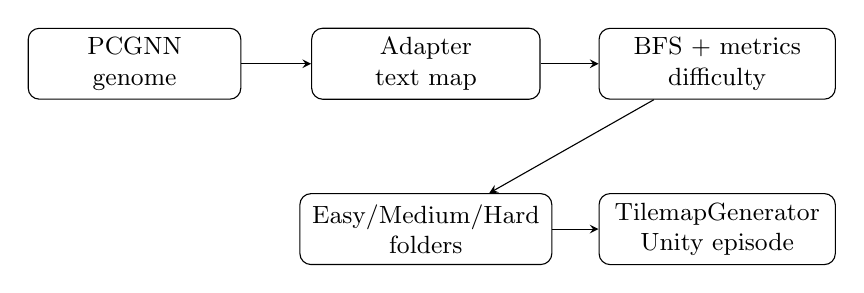
\begin{tikzpicture}[node distance=1.7cm, >=stealth, every node/.style={font=\small}]
        \node[draw, rounded corners, align=center, minimum width=2.7cm, minimum height=0.9cm] (pcgnn) {PCGNN\\genome};
        \node[draw, rounded corners, align=center, right of=pcgnn, xshift=2.0cm, minimum width=2.9cm, minimum height=0.9cm] (adapter) {Adapter\\text map};
        \node[draw, rounded corners, align=center, right of=adapter, xshift=2.0cm, minimum width=3.0cm, minimum height=0.9cm] (metric) {BFS + metrics\\difficulty};
        \node[draw, rounded corners, align=center, below of=adapter, yshift=-0.4cm, minimum width=3.2cm, minimum height=0.9cm] (tiers) {Easy/Medium/Hard\\folders};
        \node[draw, rounded corners, align=center, right of=tiers, xshift=2.0cm, minimum width=3.0cm, minimum height=0.9cm] (unity) {TilemapGenerator\\Unity episode};
        \draw[->] (pcgnn) -- (adapter);
        \draw[->] (adapter) -- (metric);
        \draw[->] (metric) -- (tiers);
        \draw[->] (tiers) -- (unity);
    \end{tikzpicture}
    \caption{Luồng sinh và tuyển chọn bản đồ bằng PCGNN trước khi đưa vào Unity}
    \label{fig:map_generation_workflow}
\end{figure}

\begin{figure}[H]
    \centering
    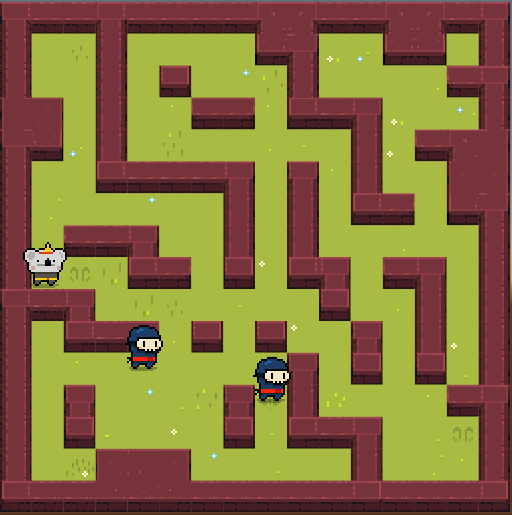
\includegraphics[width=0.72\textwidth]{figures/map_gen.png}
    \caption{Ví dụ bản đồ sau khi được dựng trong môi trường Unity từ text map}
    \label{fig:unity_generated_map_example}
\end{figure}

Độ khó bản đồ được đánh giá bằng các chỉ số hình học gồm tỷ lệ tường, độ dài đường đi ngắn nhất giữa P và E, tỷ lệ ngõ cụt, tỷ lệ vùng có thể đi tới và độ khó A*. Trong phiên bản sử dụng cho tập bản đồ hiện tại, điểm độ khó được tính theo công thức:

\begin{equation}
    \text{difficulty\_score}
    = 0.90 \times \text{wall\_ratio}
    + 0.05 \times \min(\text{path\_norm}, 1.0)
    + 0.03 \times \text{dead\_end\_ratio}
    + 0.02 \times \text{astar\_difficulty}.
    \label{eq:map_difficulty_score}
\end{equation}

Trong công thức~\ref{eq:map_difficulty_score}, \emph{wall\_ratio} được gán trọng số cao nhất vì mật độ tường ảnh hưởng trực tiếp đến không gian di chuyển và mức độ phức tạp của bản đồ. Các thành phần còn lại như độ dài đường đi, tỷ lệ ngõ cụt và độ khó A* đóng vai trò bổ trợ, giúp tinh chỉnh thứ hạng độ khó thay vì chi phối hoàn toàn kết quả phân loại. Thay vì đặt ngưỡng tuyệt đối cứng cho mọi generator, hệ thống có thể chia bản đồ theo thứ hạng tương đối: 5\% dễ nhất được đưa vào Easy, 5\% tiếp theo vào Medium và phần còn lại vào Hard. Cách chia này phù hợp với giai đoạn tuyển chọn thủ công vì người thiết kế vẫn có thể xem lại từng folder và chọn những bản đồ tốt nhất trước khi đưa sang Unity.

\textbf{Tập bản đồ đưa vào Unity.} Ở giai đoạn sinh ứng viên, batch PCGNN chính có 1000 bản đồ kích thước $14\times14$ và có thể được chia theo tỷ lệ 5/5/90 để tạo tập ứng viên Easy, Medium và Hard. Tuy nhiên, khóa luận không sử dụng toàn bộ 1000 bản đồ này trong Unity. Thay vào đó, các bản đồ được xem xét và chọn lọc theo từng mức độ khó, sau đó chỉ một tập con đại diện được gán trực tiếp cho các thí nghiệm hiện tại, gồm 5 Easy, 5 Medium và 50 Hard. Cách dùng tập con này giúp kiểm soát chất lượng bản đồ trước khi mở rộng phân loại đầy đủ: Easy và Medium đóng vai trò ``giàn giáo'' trong giai đoạn đầu, còn Hard là phân phối mục tiêu chiếm phần lớn thời gian huấn luyện.

\begin{table}[H]
    \centering
    \small
    \caption{Phân bố bản đồ đang gán trong Unity theo tier độ khó}
    \label{tab:map_split}
    \begin{tabular}{|p{2.5cm}|c|c|p{7.5cm}|}
        \hline
        \textbf{Tier} & \textbf{Số bản đồ} & \textbf{Tỷ lệ} & \textbf{Vai trò trong huấn luyện} \\
        \hline
        Easy   & 5  & 8.33\%  & Giàn giáo gradient cho giai đoạn $\sim$0--70k bước; tập nhỏ đã được chọn để agent gặp success thường xuyên. \\
        \hline
        Medium & 5  & 8.33\%  & Bước trung gian từ Easy sang Hard, dùng khoảng $\sim$70k--140k bước. \\
        \hline
        Hard   & 50 & 83.33\% & Phân phối mục tiêu, chiếm hơn 95\% thời gian huấn luyện; số lượng lớn hơn hai tier đầu để tăng đa dạng bố cục. \\
        \hline
    \end{tabular}
\end{table}

Trong Unity, TilemapGenerator không cần biết bản đồ được vẽ tay hay sinh bằng PCGNN. Thành phần này chỉ đọc text asset theo tier hiện tại, dựng tilemap và kiểm tra lại vùng có thể đi tới. Với các lesson dùng fixed spawn, TilemapGenerator ưu tiên ô sàn có độ phủ BFS tốt để tránh trường hợp player hoặc enemy bị cô lập. Với lesson dùng random spawn, player và enemy được chọn từ các ô sàn hợp lệ nhằm tăng phương sai môi trường. Hình~\ref{fig:unity_tilemap_generator_inspector} minh họa cấu hình TilemapGenerator trong Inspector, trong đó Unity đang dùng chế độ Curriculum với 5 Easy maps, 5 Medium maps và 50 Hard maps.

\begin{figure}[H]
    \centering
    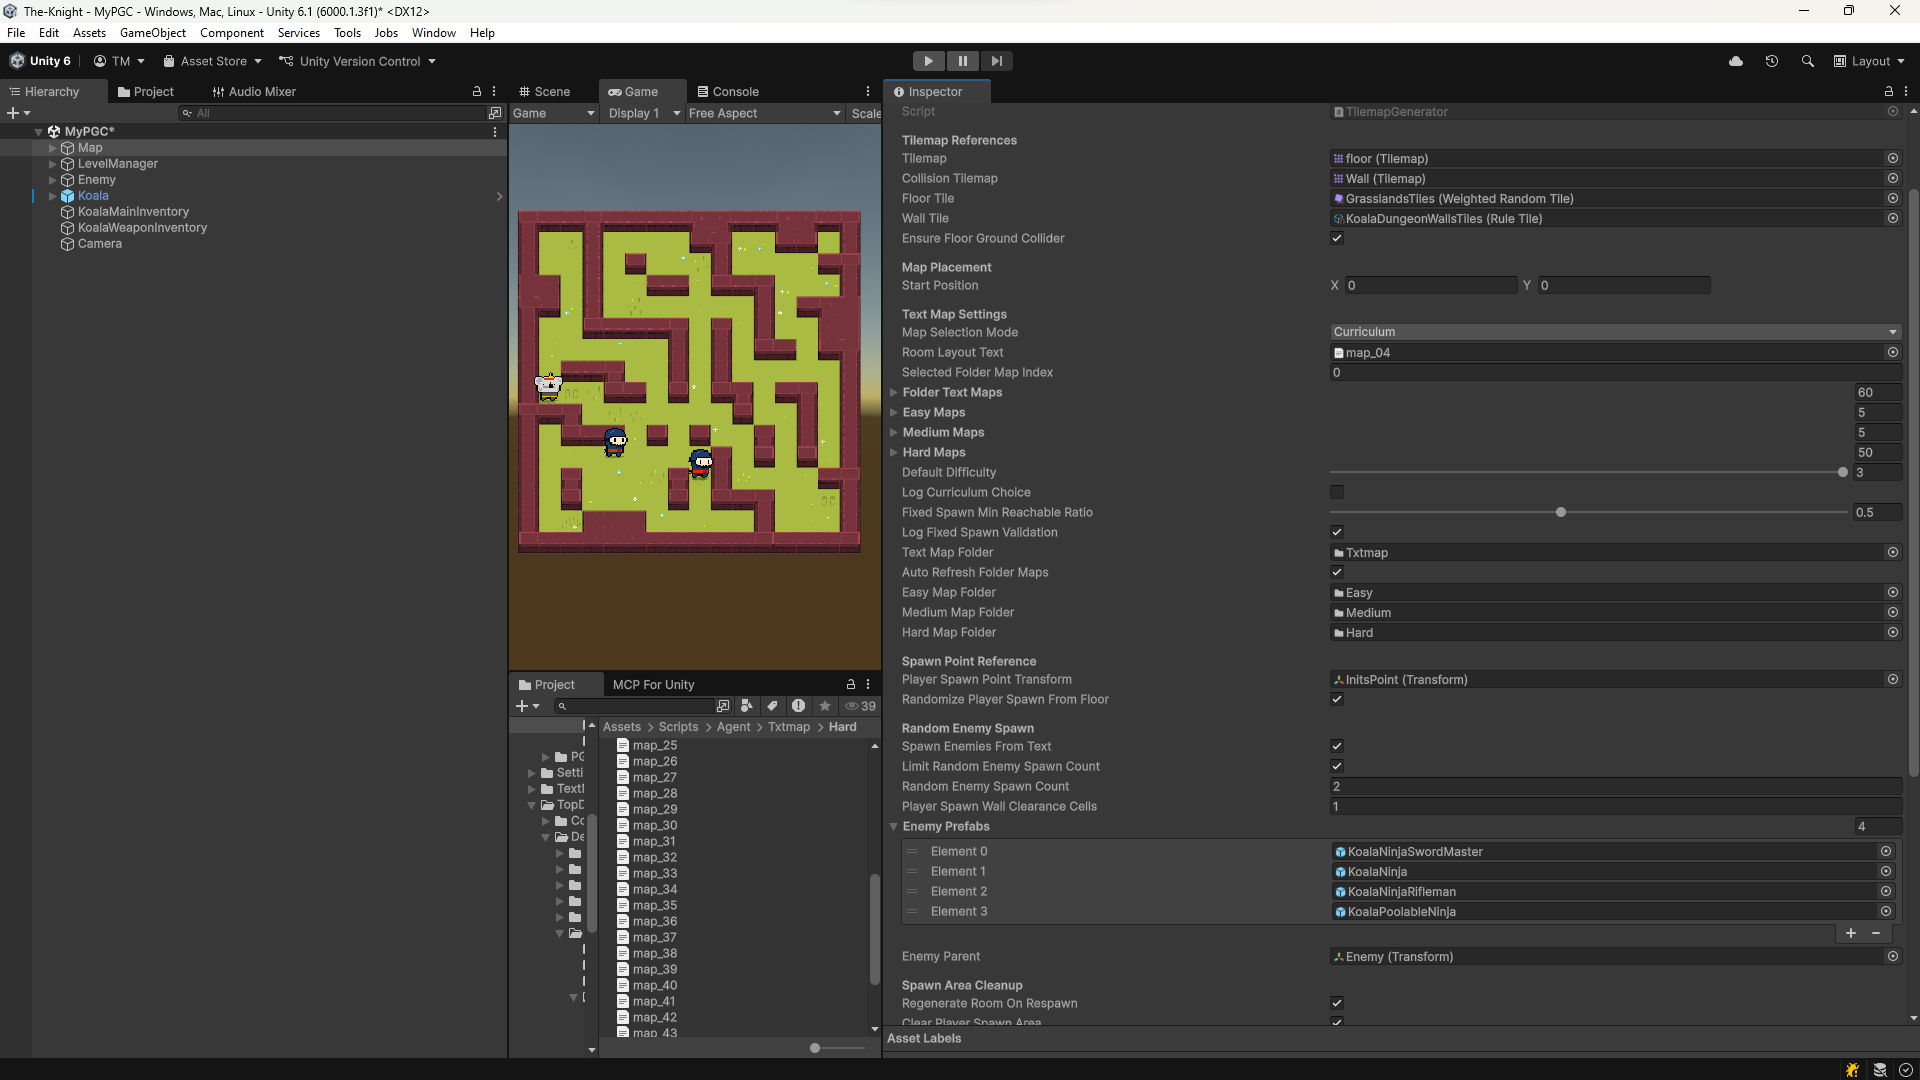
\includegraphics[width=0.98\textwidth]{figures/unity_env.png}
    \caption{Cấu hình TilemapGenerator trong Unity Inspector và ví dụ bản đồ đang được dựng trong Game view}
    \label{fig:unity_tilemap_generator_inspector}
\end{figure}

Bảng~\ref{tab:difficulty_spawn_policy} tóm tắt cách chọn bản đồ và vị trí sinh trong từng mức độ khó. Trong các run curriculum chính, tham số môi trường \emph{difficulty} do ML-Agents truyền vào quyết định cả folder bản đồ lẫn chế độ spawn. Với \emph{difficulty}=0, 1 và 2, hệ thống dùng fixed spawn: trên mỗi bản đồ, vị trí người chơi được chọn theo một quy tắc xác định và được cache lại, còn các vị trí enemy được chọn từ các ô sàn có thể đi tới từ người chơi, trải theo các mức khoảng cách trung bình để tránh việc quái luôn xuất hiện quá gần hoặc quá xa. Với \emph{difficulty}=3, hệ thống vẫn dùng tập Hard nhưng chuyển sang random spawn: người chơi và enemy được lấy ngẫu nhiên từ các ô sàn hợp lệ sau mỗi episode. Trong cấu hình huấn luyện chính, số enemy sinh ra mỗi episode được giới hạn bởi \emph{randomEnemySpawnCount}=2; nếu có nhiều prefab enemy, prefab cụ thể được lấy từ mảng \emph{enemyPrefabs}.

\begin{table}[H]
    \centering
    \small
    \caption{Chính sách chọn map và spawn theo tham số \emph{difficulty}}
    \label{tab:difficulty_spawn_policy}
    \makebox[\textwidth][c]{%
    \begin{tabular}{|c|p{2.3cm}|p{2.5cm}|p{4.0cm}|p{4.0cm}|}
        \hline
        \textbf{\emph{difficulty}} & \textbf{Tier bản đồ} & \textbf{Chế độ spawn} & \textbf{Player spawn} & \textbf{Enemy spawn} \\
        \hline
        0 & Easy & Fixed & Một ô sàn hợp lệ được chọn xác định cho từng map, ưu tiên vùng có không gian di chuyển tốt. & Tối đa 2 enemy ở các ô sàn hợp lệ, có thể đi tới từ player và phân bố ở khoảng cách trung bình. \\
        \hline
        1 & Medium & Fixed & Giữ quy tắc fixed spawn như Easy nhưng dùng tập map phức tạp hơn. & Giữ quy tắc fixed enemy spawn để giảm phương sai khi agent học bản đồ khó hơn. \\
        \hline
        2 & Hard & Fixed & Dùng tập Hard nhưng vẫn cố định spawn theo từng map. & Enemy vẫn được đặt xác định theo map để agent học kỹ năng combat trên cấu trúc khó trước. \\
        \hline
        3 & Hard & Random & Chọn ngẫu nhiên một ô sàn hợp lệ ở mỗi episode. & Chọn ngẫu nhiên tối đa 2 ô sàn hợp lệ có thể đi tới từ player, nhằm tăng khả năng khái quát hóa với spawn mới. \\
        \hline
    \end{tabular}
    }
\end{table}

Như vậy, độ khó không chỉ tăng vì bản đồ chuyển từ Easy sang Medium và Hard, mà còn tăng vì phương sai vị trí sinh được mở rộng ở lesson Hard Random. Cách tách này giúp agent học trước các kỹ năng nền như tiếp cận, né đạn và căn hướng tấn công trong môi trường ít nhiễu hơn, sau đó mới phải thích nghi với vị trí sinh thay đổi mạnh.

\section{Khung curriculum learning}

Curriculum learning được dùng để giảm độ khó khám phá ban đầu \cite{Bengio2009}. Thay vì đưa tác nhân ngay vào toàn bộ phân phối Hard, hệ thống bắt đầu từ bản đồ dễ hơn, chuyển sang Medium khi phần thưởng làm mượt vượt ngưỡng, rồi mới mở Hard. Tham số bài học được truyền qua Academy.Instance.EnvironmentParameters với tên difficulty.

\begin{figure}[H]
    \centering
    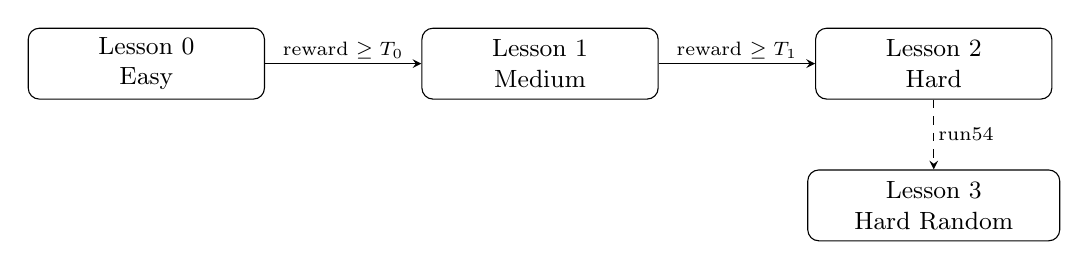
\begin{tikzpicture}[>=stealth,
        lesson/.style={draw, rounded corners, align=center, minimum width=3.0cm, minimum height=0.9cm, font=\small},
        transition/.style={font=\scriptsize, fill=white, inner sep=1.5pt}]
        \node[lesson] (easy) at (0,0) {Lesson 0\\Easy};
        \node[lesson] (medium) at (5.0,0) {Lesson 1\\Medium};
        \node[lesson] (hard) at (10.0,0) {Lesson 2\\Hard};
        \node[lesson, minimum width=3.2cm] (random) at (10.0,-1.8) {Lesson 3\\Hard Random};
        \draw[->] (easy.east) -- node[transition, above]{reward $\geq T_0$} (medium.west);
        \draw[->] (medium.east) -- node[transition, above]{reward $\geq T_1$} (hard.west);
        \draw[->, dashed] (hard.south) -- node[transition, right]{run54} (random.north);
    \end{tikzpicture}
    \caption{Cấu trúc curriculum 3-tier và biến thể 4-tier fixed-to-random}
    \label{fig:curriculum_structure}
\end{figure}

Trong run46, curriculum gồm 3 lesson: Easy, Medium và Hard. Trong run54, curriculum được mở rộng thành 4 lesson: Easy Fixed, Medium Fixed, Hard Fixed và Hard Random. Biến thể 4-tier kiểm tra giả thuyết rằng việc giảm phương sai spawn ở giai đoạn đầu có thể giúp PPO ổn định hơn trước khi chuyển sang phân phối khó hơn.

Cần phân biệt hai lớp tổ chức độ khó. Lớp thứ nhất là chia tập bản đồ PCGNN thành các folder Easy, Medium và Hard dựa trên chỉ số hình học. Lớp thứ hai là lịch chuyển lesson trong ML-Agents: trainer thay đổi tham số \emph{difficulty} khi reward làm mượt vượt ngưỡng, từ đó TilemapGenerator chọn folder bản đồ và chế độ spawn tương ứng.

\section{Kiến trúc mạng nơ-ron}

Chính sách được huấn luyện bằng PPO trong Unity ML-Agents \cite{Juliani2018}. Cấu hình baseline dùng mạng MLP actor-critic với hidden\_units=256, num\_layers=2, normalize=true. Actor head sinh phân phối xác suất cho bốn branch hành động, còn critic head ước lượng $V(s)$ để tính advantage theo GAE.

\begin{figure}[H]
    \centering
    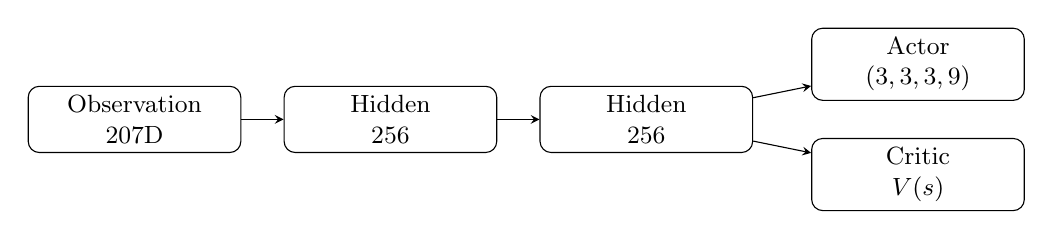
\begin{tikzpicture}[node distance=1.45cm, >=stealth, every node/.style={font=\small}]
        \node[draw, rounded corners, align=center, minimum width=2.7cm] (obs) {Observation\\207D};
        \node[draw, rounded corners, align=center, right of=obs, xshift=1.8cm, minimum width=2.7cm] (h1) {Hidden\\256};
        \node[draw, rounded corners, align=center, right of=h1, xshift=1.8cm, minimum width=2.7cm] (h2) {Hidden\\256};
        \node[draw, rounded corners, align=center, right of=h2, xshift=2.0cm, yshift=0.7cm, minimum width=2.7cm] (actor) {Actor\\$(3,3,3,9)$};
        \node[draw, rounded corners, align=center, right of=h2, xshift=2.0cm, yshift=-0.7cm, minimum width=2.7cm] (critic) {Critic\\$V(s)$};
        \draw[->] (obs) -- (h1);
        \draw[->] (h1) -- (h2);
        \draw[->] (h2) -- (actor);
        \draw[->] (h2) -- (critic);
    \end{tikzpicture}
    \caption{Kiến trúc actor-critic dùng cho CombatAgentConfig}
    \label{fig:actor_critic_architecture}
\end{figure}

Một số run ablation bổ sung bộ nhớ LSTM với memory\_size=256 và sequence\_length=64 để kiểm tra giả thuyết rằng thông tin lịch sử có thể giúp agent xử lý đạn, hồi chiêu và tình huống khuất tầm nhìn. Kết quả định lượng của các lựa chọn kiến trúc này được trình bày ở Chương~4.

\section{Cấu hình hyperparameter PPO}

Bảng~\ref{tab:ppo_hyperparams} trình bày các hyperparameter chính được sử dụng cho trainer PPO trong Unity ML-Agents \cite{Juliani2018}. Cấu hình này được giữ thống nhất giữa các run ablation từ run34 đến run54 (trừ các phần được thay đổi rõ ràng như intrinsic reward, LSTM hoặc curriculum); run55 chỉ thay đổi reward landscape chứ không thay đổi hyperparameter trainer.

\begin{table}[H]
    \centering
    \small
    \caption{Cấu hình hyperparameter chính của trainer PPO}
    \label{tab:ppo_hyperparams}
    \begin{tabular}{|p{4.0cm}|c|p{7.2cm}|}
        \hline
        \textbf{Hyperparameter} & \textbf{Giá trị} & \textbf{Ý nghĩa} \\
        \hline
        \emph{learning\_rate}      & $3{\times}10^{-4}$ & Tốc độ học của Adam optimizer; là giá trị mặc định khuyến nghị của ML-Agents cho PPO. \\
        \hline
        \emph{learning\_rate\_schedule} & linear & Giảm tuyến tính learning rate xuống 0 ở cuối quá trình huấn luyện để ổn định cập nhật giai đoạn cuối. \\
        \hline
        \emph{batch\_size}         & 1024  & Kích thước minibatch khi cập nhật policy. \\
        \hline
        \emph{buffer\_size}        & 10240 & Số bước trải nghiệm thu thập trước mỗi lần cập nhật PPO. \\
        \hline
        \emph{num\_epoch}          & 3     & Số lần lặp qua buffer trong một lần cập nhật. \\
        \hline
        $\gamma$ (\emph{gamma})    & 0.99  & Hệ số chiết khấu cho phần thưởng tương lai. \\
        \hline
        $\lambda$ (\emph{lambd})   & 0.95  & Tham số GAE cân bằng độ lệch và phương sai (Phương trình~\ref{eq:gae_formula}). \\
        \hline
        $\epsilon$ (\emph{epsilon})& 0.2   & Biên độ cắt PPO của tỷ lệ xác suất $r_t(\theta)$ (Phương trình~\ref{eq:ppo_clip}). \\
        \hline
        $\beta$ (\emph{beta})      & $5{\times}10^{-3}$ & Hệ số entropy bonus, được giảm tuyến tính để khuyến khích khám phá ban đầu. \\
        \hline
        \emph{time\_horizon}       & 64    & Số bước trước khi bootstrap value estimate khi episode chưa kết thúc. \\
        \hline
        \emph{hidden\_units}       & 256   & Số neuron của mỗi lớp ẩn trong shared MLP backbone. \\
        \hline
        \emph{num\_layers}         & 2     & Số lớp ẩn của shared MLP backbone. \\
        \hline
        \emph{normalize}           & true  & Chuẩn hóa observation theo running mean/std để ổn định gradient. \\
        \hline
        \emph{memory\_size}        & 256   & Kích thước trạng thái ẩn LSTM (chỉ áp dụng cho run42, run47). \\
        \hline
        \emph{sequence\_length}    & 64    & Độ dài chuỗi quan sát đưa vào LSTM (chỉ áp dụng cho run42, run47). \\
        \hline
        \emph{max\_steps}          & 1M / 3M & Tổng bước huấn luyện: 1M cho các run baseline (run34--42), 3M cho các run curriculum (run46+). \\
        \hline
    \end{tabular}
\end{table}

Cấu hình PPO được giữ gần mặc định để tập trung đánh giá curriculum, reward và intrinsic motivation.
